%%%%%%%%%%%%%%%%%%%%%%%%%%%%%%%%%%%%%%%%%
% Beamer Presentation
% LaTeX Template
% Version 1.0 (10/11/12)
%
% This template has been downloaded from:
% http://www.LaTeXTemplates.com
%
% License:
% CC BY-NC-SA 3.0 (http://creativecommons.org/licenses/by-nc-sa/3.0/)
%
%%%%%%%%%%%%%%%%%%%%%%%%%%%%%%%%%%%%%%%%%

%----------------------------------------------------------------------------------------
%	PACKAGES AND THEMES
%----------------------------------------------------------------------------------------

\documentclass[handout]{beamer}

\mode<presentation> {

% The Beamer class comes with a number of default slide themes
% which change the colors and layouts of slides. Below this is a list
% of all the themes, uncomment each in turn to see what they look like.

%\usetheme{default}
%\usetheme{AnnArbor}
%\usetheme{Antibes}
%\usetheme{Bergen}
%\usetheme{Berkeley}
%\usetheme{Berlin}
%\usetheme{Boadilla}
%\usetheme{CambridgeUS}
%\usetheme{Copenhagen}
%\usetheme{Darmstadt}
%\usetheme{Dresden}
%\usetheme{Frankfurt}
%\usetheme{Goettingen}
%\usetheme{Hannover}
%\usetheme{Ilmenau}
%\usetheme{JuanLesPins}
%\usetheme{Luebeck}
\usetheme{Madrid}
%\usetheme{Malmoe}
%\usetheme{Marburg}
%\usetheme{Montpellier}
%\usetheme{PaloAlto}
%\usetheme{Pittsburgh}
%\usetheme{Rochester}
%\usetheme{Singapore}
%\usetheme{Szeged}
%\usetheme{Warsaw}

% As well as themes, the Beamer class has a number of color themes
% for any slide theme. Uncomment each of these in turn to see how it
% changes the colors of your current slide theme.

%\usecolortheme{albatross}
%\usecolortheme{beaver}
%\usecolortheme{beetle}
%\usecolortheme{crane}
%\usecolortheme{dolphin}
%\usecolortheme{dove}
%\usecolortheme{fly}
%\usecolortheme{lily}
%\usecolortheme{orchid}
%\usecolortheme{rose}
%\usecolortheme{seagull}
%\usecolortheme{seahorse}
%\usecolortheme{whale}
%\usecolortheme{wolverine}

%\setbeamertemplate{footline} % To remove the footer line in all slides uncomment this line
%\setbeamertemplate{footline}[page number] % To replace the footer line in all slides with a simple slide count uncomment this line

%\setbeamertemplate{navigation symbols}{} % To remove the navigation symbols from the bottom of all slides uncomment this line
}

\usepackage{graphicx} % Allows including images
\usepackage{booktabs} % Allows the use of \toprule, \midrule and \bottomrule in tables
\usepackage{cool}
\usepackage{amsmath}
\usepackage{amssymb}
\usepackage{pseudocode}
\usepackage{bm}
\usepackage{multirow}
\usepackage{physics}
\usepackage{hyperref}
\usepackage{listings}
\usepackage{enumerate}
\usepackage{pifont}% http://ctan.org/pkg/pifont
\newcommand{\cmark}{\ding{51}}%
\newcommand{\xmark}{\ding{55}}%

\newcommand{\prob}{\mathcal{P}}
\newcommand{\rew}{\mathcal{R}}
\newcommand{\states}{\mathcal{S}}
\newcommand{\actions}{\mathcal{S}}

\DeclareMathOperator*{\argmin}{arg\,min}
\DeclareMathOperator*{\argmax}{arg\,max}

\newcommand{\bvpi}{\bm{V}^{\pi}}
\newcommand{\bvs}{\bm{V}^*}
\newcommand{\bbpi}{\bm{B}^{\pi}}
\newcommand{\bbs}{\bm{B}^*}
\newcommand{\bv}{\bm{V}}

%----------------------------------------------------------------------------------------
%	TITLE PAGE
%----------------------------------------------------------------------------------------

\title[RL Control Chapter]{A Guided Tour of \href{http://stanford.edu/~ashlearn/RLForFinanceBook/book.pdf}{\underline{\textcolor{yellow}{Chapter 10}}}: \\ Reinforcement Learning for Control} % The short title appears at the bottom of every slide, the full title is only on the title page

\author{Ashwin Rao} % Your name
\institute[Stanford] % Your institution as it will appear on the bottom of every slide, may be shorthand to save space
{ICME, Stanford University
 % Your institution for the title page
}

\date % Date, can be changed to a custom date

\begin{document}
\lstset{language=Python}  
\begin{frame}
\titlepage % Print the title page as the first slide
\end{frame}

% \begin{frame}
% \frametitle{Overview} % Table of contents slide, comment this block out to remove it
% \tableofcontents % Throughout your presentation, if you choose to use \section{} and \subsection{} commands, these will automatically be printed on this slide as an overview of your presentation
% \end{frame}

\begin{frame}
\frametitle{RL does not have access to a probability model}
\begin{itemize}[<+->]
\item DP/ADP assume access to probability model (knowledge of $\mathcal{P}_R$)
\item Often in real-world, we do not have access to these probabilities
\item Which means we'd need to {\em interact} with the {\em actual environment}
\item {Actual Environment} serves up individual experiences, not probabilities
\item Even if MDP model is available, model updates can be challenging
\item Often real-world models end up being too large or too complex
\item Sometimes estimating a {\em sampling model} is much more feasible
\item So RL interacts with either {\em actual} or {\em simulated} environment
\item Either way, we receive {\em individual experiences} of next state and reward
\item We saw how RL Prediction learns from individual experiences
\item Now we extend those ideas to RL Control: Learning Optimal VF
\item We start with Tabular RL Control
 \end{itemize}
\end{frame}

\begin{frame}
\frametitle{Let us recall the Policy Iteration algorithm}
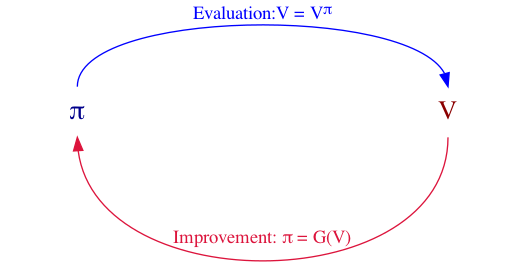
\includegraphics[width=12cm, height=5cm]{policy_iteration_loop.png}

\includegraphics[width=12cm, height=2cm]{policy_iteration_convergence.png}
\end{frame}

\begin{frame}
\frametitle{The idea of Generalized Policy Iteration (GPI)}
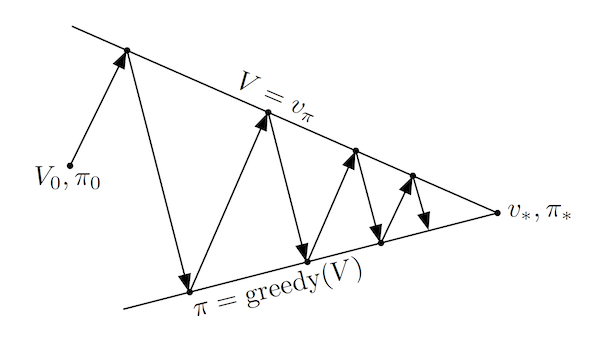
\includegraphics[width=10cm, height=5cm]{vf_policy_intersecting_lines.png}
\pause
\begin{itemize}[<+->]
\item {\em Any} Policy Evaluation method, {\em Any} Policy Improvement method
\item Policy Evaluation estimates $V^{(\pi)}$, eg: Iterative Policy Evaluation
\item Policy Improvement produces $\pi' \geq \pi$, eg: Greedy Policy Improvement
\item Policy Evaluation and Policy Improvement alternate until convergence
\end{itemize}
\end{frame}

\begin{frame}
\frametitle{Natural Idea: GPI with Tabular Monte-Carlo Evaluation}
\begin{itemize}[<+->]
\item Let us explore GPI with Tabular Monte-Carlo evaluation
\item So we will do Policy Evaluation with Tabular MC evaluation
\item And we will do the usual Greedy Policy Improvement
\item But Greedy Policy Improvement requires a model of MDP
$$\pi'(s) \leftarrow  \argmax_{a\in \mathcal{A}} \{\mathcal{R}(s,a) + \gamma \sum_{s' \in \mathcal{N}} \mathcal{P}(s,a,s') \cdot V^{\pi}(s') \}$$
\item However, it works if we were working with Action-Value Function
$$\pi'(s) \leftarrow \argmax_{a\in \mathcal{A}} Q^{\pi}(s,a)$$
\item This means: Policy Evaluation for Action-Value Function $Q^{\pi}(s,a)$
\item Following a policy $\pi$, update Q-value for each $(S_t,A_t)$ each episode:
$$Count(S_t,A_t) \leftarrow Count(S_t,A_t) + 1$$
$$Q(S_t,A_t) \leftarrow Q(S_t,A_t) + \frac 1 {Count(S_t, A_t)} \cdot (G_t - Q(S_t,A_t))$$
\end{itemize}
\end{frame}

\begin{frame}
\frametitle{$\epsilon$-Greedy Policy Improvement}
\begin{itemize}[<+->]
\item A full Policy Evaluation with MC takes too long
\item So we typically improve policy after each episode
\item This can lead to some actions not being tried enough
\item Which can lead to premature (greedy) domination of an action
\item Which can lead to other actions getting ``locked-out''
\item Same as {\em Explore v/s Exploit} dilemma of Multi-Armed Bandit problem
\item Simple solution: Perform an $\epsilon$-Greedy Policy Improvement
\item All $|\mathcal{A}|$ actions are tried with non-zero probability (for each state)
\item Pick the greedy action with probability $1-\epsilon$
\item With probability $\epsilon$, randomly choose one of the $|\mathcal{A}|$ actions
$$\text{Stochastic Policy } \pi(s,a) = 
\begin{cases}
\frac {\epsilon} {|\mathcal{A}|} + 1 - \epsilon & \text{ if } a = \argmax_{b \in \mathcal{A}} Q(s, b) \\
\frac {\epsilon} {|\mathcal{A}|} & \text{ otherwise}
\end{cases}
$$
\end{itemize}
\end{frame}


\begin{frame}
\frametitle{$\epsilon$-Greedy improves the policy}
\pause
\begin{theorem}
For any $\epsilon$-greedy policy $\pi$, the $\epsilon$-greedy policy $\pi'$ with respect to $Q^{\pi}$ is an improvement, i.e., $\bm{V}^{\pi'}(s) \geq \bm{V}^{\pi}(s)$ for all $s \in \mathcal{N}$.
\end{theorem}
\pause
\begin{itemize}[<+->]
\item Applying $\bm{B}^{\pi'}$ repeatedly (starting with $\bvpi$) converges to $\bm{V}^{\pi'}$:
$$\lim_{i\rightarrow \infty} (\bm{B}^{\pi'})^i(\bvpi) = \bm{V}^{\pi'}$$
\item So the proof is complete if we prove that:
$$(\bm{B}^{\pi'})^{i+1}(\bvpi) \geq (\bm{B}^{\pi'})^i(\bvpi) \text{ for all } i = 0, 1, 2, \ldots$$
\item Increasing tower of Value Functions $[(\bm{B}^{\pi'})^i(\bvpi)|i = 0, 1, 2, \ldots]$ with repeated applications of $\bm{B}^{\pi'}$
\end{itemize}
\end{frame}

\begin{frame}
\frametitle{Proof of $\epsilon$-Greedy improving the policy}
\pause
To prove base case (proof by induction), note: $\bm{B}^{\pi'}(\bvpi)(s)  = Q^{\pi}(s, \pi'(s))$
\pause
\begin{align*}
Q^{\pi}(s, \pi'(s)) & = \sum_{a \in \mathcal{A}} \pi'(s, a) \cdot Q^{\pi}(s,a) \\
& = \frac {\epsilon} {|\mathcal{A}|} \cdot \sum_{a \in \mathcal{A}} Q^{\pi}(s,a) + (1 - \epsilon) \cdot \max_{a \in \mathcal{A}} Q^{\pi}(s,a) \\
& \geq \frac {\epsilon} {|\mathcal{A}|} \cdot \sum_{a \in \mathcal{A}} Q^{\pi}(s,a) + (1 - \epsilon) \cdot \sum_{a \in \mathcal{A}} \frac {\pi(s,a) - \frac {\epsilon} {|\mathcal{A}|}} {1 - \epsilon} \cdot Q^{\pi}(s,a) \\
& = \sum_{a \in \mathcal{A}} \pi(s,a) \cdot Q^{\pi}(s,a) = \bm{V}^{\pi}(s)
\end{align*}
\pause
Induction step is proved by monotonicity of $\bm{B}^{\pi}$ operator (for any $\pi$):
\pause
$$\text{Monotonicity Property of } \bm{B}^{\pi}: \bm{X} \geq \bm{Y} \Rightarrow \bm{B}^{\pi}(\bm{X}) \geq \bm{B}^{\pi}(\bm{Y})$$
\pause
$$\text{So } (\bm{B}^{\pi'})^{i+1}(\bvpi) \geq (\bm{B}^{\pi'})^i(\bvpi) \Rightarrow (\bm{B}^{\pi'})^{i+2}(\bvpi) \geq (\bm{B}^{\pi'})^{i+1}(\bvpi)$$
\qed
\end{frame}


\begin{frame}
\frametitle{GLIE}
\pause
\begin{definition}
{\em Greedy in the Limit with Infinite Exploration} (GLIE):
\pause
\begin{itemize}[<+->]
\item  All state-action pairs are explored infinitely many times
$$\lim_{k \rightarrow \infty} N_k(s,a) = \infty$$
\item The policy converges to a greedy policy
$$\lim_{k\rightarrow \infty} \pi_k(s,a) = \mathbb{I}_{a = \argmax_{b \in \mathcal{A}} Q(s,b)}$$
\end{itemize}
\end{definition}
\pause
$\epsilon$-greedy can be made GLIE if $\epsilon$ is reduced as: $\epsilon_k = \frac 1 k$
\end{frame}

\begin{frame}
\frametitle{GLIE Tabular Monte-Carlo Control}
\pause
\begin{itemize}[<+->]
\item  Sample $k$-th episode using $\pi$: $\{S_0, A_0, R_1, S_1, A_1, \ldots, R_T, S_T\} \sim \pi$
\item For each state $S_t$ and action $A_t$ in the episode:
$$Count(S_t,A_t) \leftarrow Count(S_t,A_t) + 1$$
$$Q(S_t,A_t) \leftarrow Q(S_t,A_t) + \frac 1 {Count(S_t, A_t)} \cdot (G_t - Q(S_t,A_t))$$
\item Improve policy at end of episode based on updated $Q$-Value function:
$$\epsilon \leftarrow \frac 1 k$$
$$\pi \leftarrow \epsilon \text{-greedy}(Q)$$
\end{itemize}
\pause
\begin{theorem}
GLIE Tabular Monte-Carlo Control converges to the Optimal Action-Value function: $Q(s,a) \rightarrow Q^*(s,a)$.
\end{theorem}
\end{frame}


\begin{frame}
\frametitle{MC versus TD Control}
\pause
\begin{itemize}[<+->]
\item TD learning has several advantages over MC learning:
\begin{itemize}[<+->]
\item Lower variance
\item Online
\item Can work with incomplete traces or continuing traces
\item Generic interface of \lstinline{Iterable} of atomic experiences allows for serving up atomic experiences in any order (eg: atomic experience replays)
\end{itemize}
\pause
\item So use TD instead of MC in our Control loop
\pause
\begin{itemize}[<+->]
\item Apply TD to $Q(S,A)$ (instead of $V(S)$)
\item Use $\epsilon$-greedy Policy Improvement
\item Update $Q(S,A)$ after each {\em atomic experience}
\item $\epsilon$-greedy policy automatically updated after each atomic experience
\end{itemize}
\end{itemize}
\end{frame}

\begin{frame}
\frametitle{Tabular SARSA Algorithm}
\begin{itemize}[<+->]
\item Tabular SARSA is our first TD Control algorithm
\item Like Tabular MC Control, Policy Improvement is $\epsilon$-greedy
\item But here Policy Evaluation is with a TD target, as below:
$$Q(S_t,A_t) \leftarrow Q(S_t,A_t) + \alpha \cdot (R_{t+1} + \gamma \cdot Q(S_{t+1}, A_{t+1}) - Q(S_t,A_t))$$
\item Note that $Q(S,A)$ is updated after each atomic experience
\item $\epsilon$-greedy policy automatically updated after each atomic experience
\item Action $A_t$ is chosen from State $S_t$ based on $\epsilon$-greedy policy
\item Action $A_{t+1}$ is chosen from State $S_{t+1}$ based on $\epsilon$-greedy policy
\item Note: Instead of $\epsilon$-greedy, we could employ a more sophisticated exploratory policy derived from $Q$-value function ($\epsilon$-greedy is just our default simple exploratory policy derived from $Q$-value function)
\end{itemize}
\end{frame}

\begin{frame}
\frametitle{SARSA Visualization}
\centerline{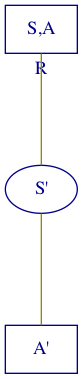
\includegraphics[width=2cm, height=8cm]{sarsa.png}}
\end{frame}


\begin{frame}
\frametitle{Convergence of Tabular SARSA}
\pause
\begin{theorem}
Tabular SARSA converges to the Optimal Action-Value function, $Q(s,a) \rightarrow Q^*(s,a)$, under the following conditions:
\begin{itemize}[<+->]
\item GLIE sequence of policies $\pi_t(s,a)$
\item Robbins-Monro sequence of step-sizes $\alpha_t$
$$\sum_{t=1}^{\infty} \alpha_t = \infty$$
$$\sum_{t=1}^{\infty} \alpha_t^2 < \infty$$
\end{itemize}
\end{theorem}
\end{frame}


\begin{frame}
\frametitle{Tabular $n$-step SARSA}
\pause
\begin{itemize}[<+->]
\item Tabular SARSA bootstraps the $Q$-Value Function with update:
$$Q(S_t, A_t) \leftarrow Q(S_t, A_t) + \alpha (R_{t+1} + \gamma Q(S_{t+1}, A_{t+1}) - Q(S_t, A_t))$$
\item So it's natural to extend this to bootstrapping with 2 steps ahead:
$$Q(S_t, A_t) \leftarrow Q(S_t, A_t) + \alpha (R_{t+1} + \gamma R_{t+2} + \gamma^2 Q(S_{t+2}, A_{t+2})- Q(S_t, A_t))$$
\item Generalize to bootstrapping with $n \geq 1$ time steps ahead:
$$Q(S_t, A_t) \leftarrow Q(S_t, A_t) + \alpha (G_{t,n} - Q(S_t, A_t))$$
\item $G_{t,n}$ (call it $n$-step bootstrapped return) is defined as:
\begin{align*}
G_{t,n} & = \sum_{i=t+1}^{t+n} \gamma^{i-t-1} \cdot R_i  + \gamma^n \cdot Q(S_{t+n}, A_{t+n}) \\
& = R_{t+1} + \gamma \cdot R_{t+2} + \ldots + \gamma^{n-1} \cdot R_{t+n} + \gamma^n \cdot Q(S_{t+n}, A_{t+n})
\end{align*}
\end{itemize}
\end{frame}

\begin{frame}
\frametitle{Tabular $\lambda$-Return SARSA}
\pause
\begin{itemize}[<+->]
\item Instead of $G_{t,n}$, a valid target is a weighted-average target:
$$\sum_{n=1}^N u_n \cdot G_{t,n} + u \cdot G_t \text{ where } u + \sum_{n=1}^N u_n = 1$$
\item Any of the $u_n$ or $u$ can be 0, as long as they all sum up to 1
\item The $\lambda$-Return target is a special case of weights $u_n$ and $u$
$$u_n = (1 - \lambda) \cdot \lambda^{n-1} \text{ for all } n = 1, \ldots, T-t-1$$
$$u_n = 0 \text{ for all } n \geq T-t \text{ and } u = \lambda^{T-t-1}$$
\item We denote the $\lambda$-Return target as $G_t^{(\lambda)}$, defined as:
$$G_t^{(\lambda)} = (1-\lambda) \cdot \sum_{n=1}^{T-t-1} \lambda^{n-1} \cdot G_{t,n} + \lambda^{T-t-1} \cdot G_t$$
$$Q(S_t, A_t) \leftarrow Q(S_t, A_t) + \alpha \cdot (G_t^{(\lambda)} - Q(S_t, A_t))$$
\end{itemize}
\end{frame}

\begin{frame}
\frametitle{Tabular SARSA($\lambda$)}
\pause
\begin{itemize}[<+->]
\item $\lambda$ can be tuned from SARSA ($\lambda=0$) to MC Control ($\lambda=1$)
\item Note that for $\lambda > 0$, $\lambda$-Return SARSA is an Offline Algorithm
\item SARSA($\lambda$) is online ``version'' of $\lambda$-Return SARSA
\item Similar to TD($\lambda$) for Prediction, SARSA($\lambda$) uses Eligibility Traces
 \item Eligibility Trace for a given trace experience at time $t$ is a function
$$E_t: \mathcal{N} \times \mathcal{A} \rightarrow \mathbb{R}_{\geq 0}$$
$$E_0(s, a) = 0, \text{ for all } s \in \mathcal{N}, a \in \mathcal{A}$$
$$E_t(s, a) = \gamma \cdot \lambda \cdot E_{t-1}(s, a) + \mathbb{I}_{S_t=s, A_t=a}, \text{ for all } s \in \mathcal{N}, a \in \mathcal{A}, \text{ for all } t$$
\item Tabular SARSA($\lambda$) performs following update at each time step $t$ in each trace experience (for each $s \in \mathcal{N}, a \in \mathcal{A}$):
$$Q(s, a) \leftarrow Q(s, a) + \alpha \cdot (R_{t+1} + \gamma \cdot Q(S_{t+1}, A_{t+1}) - Q(S_t, A_t)) \cdot E_t(s, a)$$
\end{itemize}
\end{frame}

\begin{frame}
\frametitle{Off-Policy Learning}
\pause
\begin{itemize}[<+->]
\item Estimate VF for {\em target policy} $\pi$  while following {\em behavior policy} $\mu$
$$\{S_0, A_0, R_1, S_1, A_1, \ldots, R_T, S_T\} \sim \mu$$
\item Why is this important?
\begin{itemize}[<+->]
\item Learning from observing  humans or other agents
\item Re-use experience generated from  old policies  $\pi_1, \pi_2, \ldots, \pi_{t-1}$
\item Learn about {\em optimal} policy while following {\em exploratory} policy
\item Learn about {\em multiple} policies while following {\em one} policy
\end{itemize}
\end{itemize}
\end{frame}

\begin{frame}
\frametitle{Importance Sampling for Off-Policy Learning}
\pause
\begin{itemize}[<+->]
\item Importance Sampling refers to methods to estimate properties of a distribution $P$, given access to samples from a different distribution $Q$
\item We can calculate $\mathbb{E}_{X\sim P}[f(X)]$ given samples from $Q$ as follows:
\begin{align*}
\mathbb{E}_{X\sim P}[f(X)] & = \sum P(X) \cdot f(X) \\
& = \sum Q(X) \cdot \frac {P(X)} {Q(X)} \cdot f(X) \\
& = \mathbb{E}_{X \sim Q}[\frac {P(X)} {Q(X)} \cdot f(X)]
\end{align*}
\end{itemize}
\end{frame}

\begin{frame}
\frametitle{Importance Sampling for Off-Policy Monte-Carlo}
\pause
\begin{itemize}[<+->]
\item Use returns generated from $\mu$ to estimate Value Function for $\pi$
\item Weight return $G_t$ according to similarity between policies
\item Multiply importance sampling corrections along whole episode
$$G_t^{\pi / \mu} = \frac {\pi(S_t, A_t)} {\mu(S_t, A_t)} \cdot  \frac {\pi(S_{t+1}, A_{t+1})} {\mu(S_{t+1}, A_{t+1})} \cdots \frac {\pi(S_T, A_t)} {\mu(S_T, A_T)} \cdot G_t$$
\item Update value towards {\em corrected} return
$$V(S_t) \leftarrow V(S_t) + \alpha \cdot (G_t^{\pi / \mu} - V(S_t))$$
\item Likewise for $Q$-Value Function for MC Control
\item Note: We cannot use this method if $\mu$ is zero when $\pi$ is non-zero
\item Importance sampling can dramatically increase variance
\end{itemize}
\end{frame}

\begin{frame}
\frametitle{Importance Sampling for Off-Policy Temporal-Difference}
\pause
\begin{itemize}[<+->]
\item  Use TD targets generated from $\mu$ to evaluate Value Function for $\pi$
\item Weight TD target $R + \gamma \cdot V(S')$ with importance sampling
\item Here we only need a single importance sampling correction
$$V(S_t) \leftarrow V(S_t) + \alpha \cdot ( \frac {\pi(S_t, A_t)} {\mu(S_t, A_t)} \cdot (R_{t+1} + \gamma \cdot V(S_{t+1})) - V(S_t))$$
\item Likewise for $Q$-Value Function for TD Control
\item This has much lower variance than MC importance sampling
\item Policies only need to be similar over a single step
\end{itemize}
\end{frame}

\begin{frame}
\frametitle{Tabular Q-Learning}
\pause
\begin{itemize}[<+->]
\item We now consider off-policy learning of action-values $Q(s,a)$
\item {\bf No} importance sampling is required
\item The next action is chosen using behavior policy $A_{t+1} \sim \mu(S_t,\cdot)$
\item But we consider an alternative successor action $A' \sim \pi(S_t, \cdot)$
\item Update $Q(S_t, A_t)$ towards value of alternative action
$$Q(S_t, A_t) \leftarrow Q(S_t, A_t) + \alpha \cdot (R_{t+1} + \gamma \cdot Q(S_{t+1}, A') - Q(S_t, A_t))$$ 
\end{itemize}
\end{frame}

\begin{frame}
\frametitle{Off-Policy Control with Tabular Q-Learning}
\pause
\begin{itemize}[<+->]
\item We now allow both behavior and target policies to {\bf improve}
\item The target (deterministic) policy $\pi_D$ is {\bf greedy} w.r.t $Q$-Value Function
$$\pi_D(S_{t+1}) = \argmax_{a' \in \mathcal{A}} Q(S_{t+1}, a')$$
\item The behavior policy $\mu$ is also improving, eg: $\epsilon$-greedy w.r.t. $Q$
\item The $Q$-learning target then simplifies to:
\begin{align*}
& R_{t+1} + \gamma \cdot Q(S_{t+1}, A') \\
= & R_{t+1} + \gamma \cdot Q(S_{t+1}, \argmax_{a' \in \mathcal{A}} Q(S_{t+1}, a')) \\
= & R_{t+1} + \gamma \cdot \max_{a' \in \mathcal{A}} Q(S_{t+1}, a')
\end{align*}
\item Thus the update to $Q$-Value Function after each atomic experience is:
$$Q(S_t, A_t) \leftarrow Q(S_t, A_t) + \alpha \cdot (R_{t+1} + \gamma \cdot \max_{a' \in \mathcal{A}} Q(S_{t+1}, a') - Q(S_t, A_t))$$
\end{itemize}
\end{frame}

\begin{frame}
\frametitle{Tabular Q-Learning Control Algorithm}
\pause
\begin{theorem}
Tabular Q-Learning Control converges to the Optimal Action-Value Function, $Q(s,a) \rightarrow Q^*(s,a)$
\end{theorem}
\end{frame}

\begin{frame}
\frametitle{Q-Learning Control Visualization}
\centerline{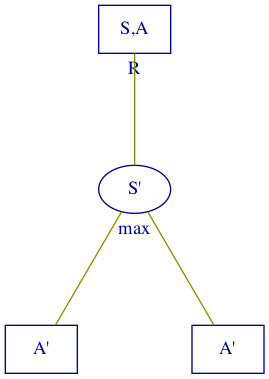
\includegraphics[width=4cm, height=8cm]{q_learning.png}}
\end{frame}

\begin{frame}
\frametitle{RL Control with Function Approximation}
\pause
\begin{itemize}[<+->]
\item Natural extension of Tabular Control to function approximations
\item Instead of parameterized approximation $V(s; \bm{w})$, we have $Q(s,a;\bm{w})$
\item GPI's Policy Evaluation is Approximate $Q$-Value Policy Evaluation
\item Loss Function for $Q(s,a;\bm{w})$ estimate relative to appropriate return
\item For MC Control, the loss function for $(S_t,A_t)$ in an episode is:
$$\mathcal{L}_{(S_t,A_t,G_t)}(\bm{w}) = \frac 1 2 \cdot (Q(S_t,A_t;\bm{w}) - G_t)^2$$
\item Therefore, the gradient of the loss function for this $(S_t,A_t)$ is:
$$\nabla_{\bm{w}} \mathcal{L}_{(S_t,A_t,G_t)}(\bm{w}) = (Q(S_t,A_t;\bm{w}) - G_t) \cdot \nabla_{\bm{w}} Q(S_t,A_t;\bm{w})$$
\item Therefore, parameters update for this $(S_t,A_t)$ at episode-end is:
$$\Delta \bm{w} = \alpha \cdot (G_t - Q(S_t,A_t;\bm{w})) \cdot \nabla_{\bm{w}} Q(S_t,A_t;\bm{w})$$
\item $\epsilon$-greedy policy improvement is automatic from updated $Q$ estimate
\end{itemize}
\end{frame}

\begin{frame}
\frametitle{Bootstrapped Control with Function Approximation}
\pause
\begin{itemize}[<+->]
\item For SARSA, parameters update after each atomic experience:
$$\Delta \bm{w} = \alpha \cdot (R_{t+1} + \gamma \cdot Q(S_{t+1},A_{t+1};\bm{w}) - Q(S_t,A_t;\bm{w})) \cdot \nabla_{\bm{w}} Q(S_t,A_t;\bm{w})$$
\item For Q-Learning, parameters update after each atomic experience:
$$\Delta \bm{w} = \alpha \cdot (R_{t+1} + \gamma \cdot \max_{a' \in \mathcal{A}} Q(S_{t+1},a';\bm{w}) - Q(S_t,A_t;\bm{w})) \cdot \nabla_{\bm{w}} Q(S_t,A_t;\bm{w})$$
\item For offline $\lambda$-Return Control, parameters update at episode-end:
$$\Delta \bm{w} = \alpha \cdot (G_t^{(\lambda)} - Q(S_t,A_t;\bm{w})) \cdot \nabla_{\bm{w}} Q(S_t,A_t;\bm{w})$$
\item For online SARSA($\lambda$), update after each atomic experience:
$$\delta_t = R_{t+1} + \gamma \cdot Q(S_{t+1},A_{t+1};\bm{w}) - Q(S_t,A_t;\bm{w})$$
$$\bm{E}_t = \gamma \lambda \cdot \bm{E}_{t-1} + \nabla_{\bm{w}} Q(S_t,A_t;\bm{w})$$
$$\Delta \bm{w} = \alpha \cdot \delta_t \cdot \bm{E}_t$$
\item $\epsilon$-greedy policy improvement is automatic from updated $Q$ estimate
\end{itemize}
\end{frame}

\begin{frame}
\frametitle{Relationship between DP and TD}
\pause
      \begin{tabular}{c|c|c}
      & {\bf Full Backup (DP)} & {\bf Sample Backup (TD)} \\ \hline
       Bellman Expectation & 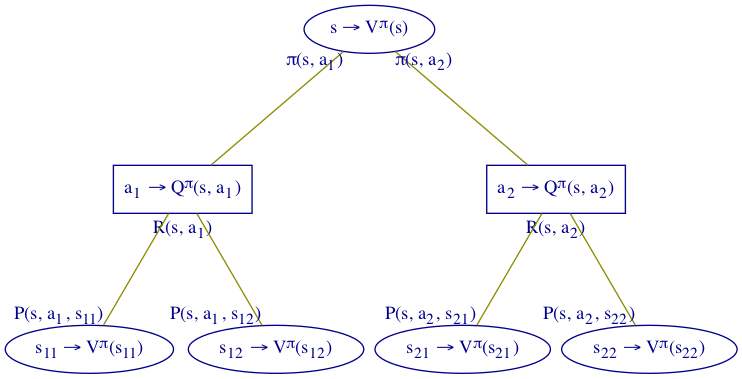
\includegraphics[width=3.0cm, height=1.9cm]{mdp_bellman_policy_tree_vv.png}  & 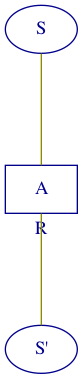
\includegraphics[width=0.5cm, height=1.9cm]{td.png} \\
               Equation for $V^{\pi}(s)$ & Iterative Policy Evaluation & TD Learning \\ \hline
        Bellman Expectation & 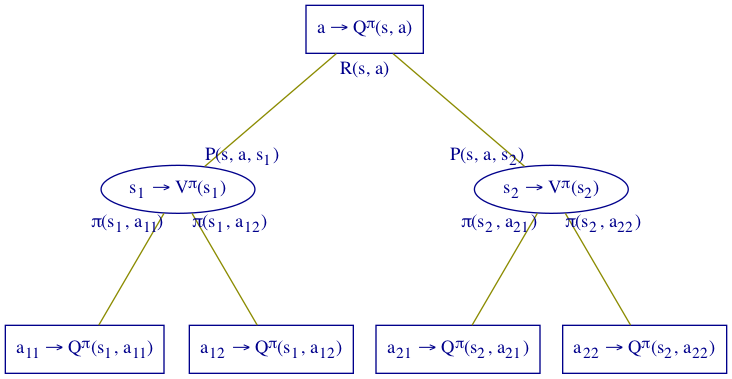
\includegraphics[width=3.0cm, height=1.9cm]{mdp_bellman_policy_tree_qq.png} & 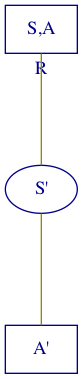
\includegraphics[width=0.5cm, height=1.9cm]{sarsa.png} \\
               Equation for $Q^{\pi}(s, a)$ & Q-Policy Iteration & SARSA \\ \hline
          Bellman Optimality & 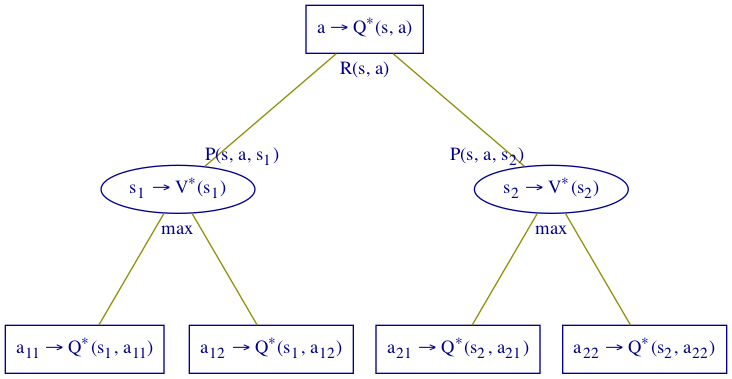
\includegraphics[width=3.0cm, height=1.9cm]{mdp_bellman_opt_tree_qq.png} & 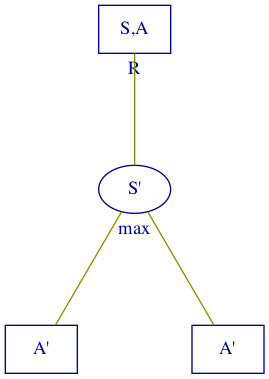
\includegraphics[width=1.5cm, height=1.9cm]{q_learning.png} \\
               Equation for $Q^*(s, a)$ & Q-Value Iteration & Q-Learning \\         
      \end{tabular}  
\end{frame}

\begin{frame}
\frametitle{Relationship between DP and TD}
\pause
\begin{center}
      \begin{tabular}{c|c}
      {\bf Full Backup (DP)} & {\bf Sample Backup (TD)} \\ \hline
       Iterative Policy Evaluation: $V(S)$ update & TD Learning: $V(S)$ update \\
       $\mathbb{E}[R + \gamma V(S')|S]$ & sample $R + \gamma V(S')$ \\ \hline
      Q-Policy Evaluation: $Q(S,A)$ update & SARSA: $Q(S,A)$ update \\
       $\mathbb{E}[R + \gamma Q(S',A')|S,A]$ & sample $R + \gamma Q(S',A')$ \\ \hline
       Q-Value Iteration: $Q(S,A)$ update & Q-Learning: $Q(S,A)$ update \\
       $\mathbb{E}[R + \gamma \max_{a'} Q(S',a')|S,A]$ & sample $R + \gamma \max_{a' } Q(S',a')$ \\ \hline
      \end{tabular} 
\end{center}      
\end{frame}

\begin{frame}
\frametitle{Convergence of Prediction Algorithms}
\pause
\begin{center}
      \begin{tabular}{ccccc}
      \hline
      On/Off Policy & Algorithm & Tabular & Linear & Non-Linear \\ \hline
      \multirow{3}{*}{On-Policy} & MC & \cmark & \cmark & \cmark \\
      & TD(0) & \cmark & \cmark & \xmark \\
      & TD($\lambda$) & \cmark & \cmark & \xmark \\ \hline
      \multirow{3}{*}{Off-Policy} & MC & \cmark & \cmark & \cmark \\
      & TD(0) & \cmark & \xmark & \xmark \\
      & TD($\lambda$) & \cmark & \xmark & \xmark \\ \hline
      \end{tabular}
\end{center}      
\end{frame}

\begin{frame}
\frametitle{Gradient Temporal-Difference Learning}
\pause
\begin{itemize}[<+->]
\item TD does not follow the gradient of {\em any} objective function
\item This is why TD can diverge:
\begin{itemize}[<+->]
\item when running off-policy, or
\item when using non-linear function approximation
\end{itemize}
\item {\bf Gradient TD} follows true gradient of projected Bellman Error
\end{itemize}
\pause
\begin{center}
      \begin{tabular}{ccccc}
      \hline
      On/Off Policy & Algorithm & Tabular & Linear & Non-Linear \\ \hline
      \multirow{4}{*}{On-Policy} & MC & \cmark & \cmark & \cmark \\
      & TD & \cmark & \cmark & \xmark \\
      & {\bf Gradient TD} & {\bf \cmark} & {\bf \cmark} & {\bf \cmark} \\ \hline
      \multirow{4}{*}{Off-Policy} & MC & \cmark & \cmark & \cmark \\
      & TD & \cmark & \xmark & \xmark \\
      & {\bf Gradient TD} & {\bf \cmark} & {\bf \cmark} & {\bf \cmark} \\ \hline
      \end{tabular} 
\end{center}      
\end{frame}

\begin{frame}
\frametitle{Convergence of Control Algorithms}
\pause
\begin{center}
      \begin{tabular}{cccc}
      \hline
      Algorithm & Tabular & Linear & Non-Linear \\ \hline
      MC Control & \cmark & ( \cmark ) & \xmark \\
      SARSA & \cmark & ( \cmark ) & \xmark \\ 
      Q-Learning & \cmark & \xmark & \xmark \\
      Gradient Q-Learning & \cmark & \cmark & \xmark \\ \hline
      \end{tabular}
 \end{center}     
  \pause
  ( \cmark ) means it chatters around near-optimal Value Function   
\end{frame}

\begin{frame}
\frametitle{Key Takeaways from this Chapter}
\pause
\begin{itemize}[<+->]
\item RL Control is based on the idea of Generalized Policy Iteration (GPI)
\begin{itemize}[<+->]
\item Policy Evaluation with $Q$-Value Function (instead of $V$)
\item Improved Policy needs to be exploratory, eg: $\epsilon$-greedy
\end{itemize}
\item On-Policy versus Off-Policy
\item Deadly Triad := [Bootstrapping, Function Approximation, Off-Policy]
\end{itemize}
\end{frame}


\end{document}